\documentclass{beamer}

\usepackage[utf8]{inputenc}
\usepackage{graphicx}
\usepackage{xcolor,colortbl}
\usepackage{subfigure}
\usepackage{hyperref}
%\usepackage{columns}
\usepackage{default}
\usetheme{Frankfurt}
\usecolortheme{seahorse}
\usepackage{listings}
\lstset{
    tabsize=4,
    rulecolor=,
    language=Python,
    basicstyle=\scriptsize,
    upquote=true,
    aboveskip={1.5\baselineskip},
    columns=fixed,
    showstringspaces=false,
    extendedchars=true,
    breaklines=true,
    prebreak = \raisebox{0ex}[0ex][0ex]{\ensuremath{\hookleftarrow}},
    frame=single,
    showtabs=false,
    showspaces=false,
    showstringspaces=false,
    identifierstyle=\ttfamily,
    keywordstyle=\color[rgb]{0,0,1},
    commentstyle=\color[rgb]{0.133,0.545,0.133},
    stringstyle=\color[rgb]{0.627,0.126,0.941},
}

\setbeamertemplate{footline}[page number]


%\usecolortheme{whale}
%\centerline{
\includegraphics[scale=0.4]{../images/easy_elua_logo}}


\title{Projet innovant RICM4: Easy-eLua}
\author{Elizabeth \textsc{Paz} \\ Salem \textsc{Harrache}}
\institute{Polytech'Grenoble \\
Olivier \textsc{Richard} \\
Didier \textsc{Donsez} \\
}

\author[Elizabeth Paz, Salem Harrache]
{Elizabeth Paz \and Salem Harrache}

\pgfdeclareimage[height=1cm]{university-logo}{../images/polytech.png}
\logo{\pgfuseimage{university-logo}}
\date{27 Avril 2012}

\begin{document}

\begin{frame}
\begin{center}

\includegraphics[scale=0.4]{../images/easy_elua_logo}
\end{center}
\titlepage
\end{frame}

\begin{frame}
\frametitle{Sommaire}
\tableofcontents
\end{frame}

\section{Introduction}
\subsection{Présentation carte STM32F4-DISCOVERY}
\begin{frame}
\frametitle{Introduction : Présentation carte STM32F4-DISCOVERY}
Partie Elizabeth

Note salem : présenter brivement les caracteristiques et puis finir sur le fait que
c'est compliqué de programmer dessus pour un novice
\begin{center}
 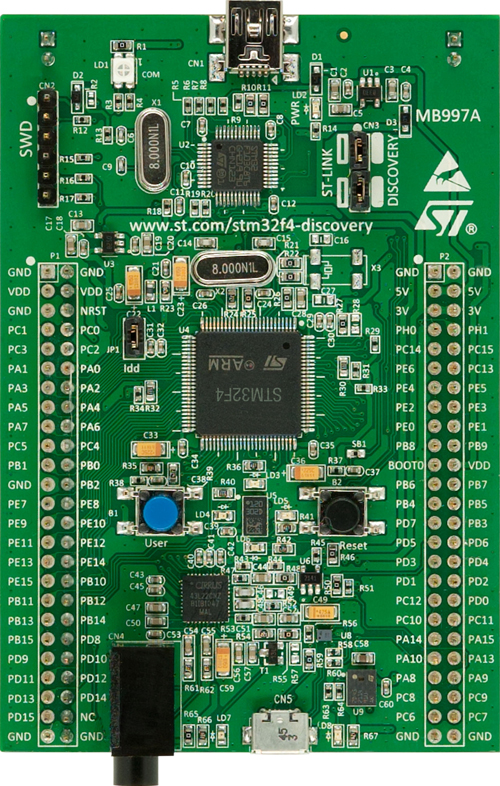
\includegraphics[scale=0.1]{../images/stm32f4_discovery.jpg}
\end{center}
\end{frame}

\subsection{Présentation Arduino}
\begin{frame}
\frametitle{Introduction : Présentation Arduino}
Partie Elizabeth
Note salem : Le site est bien fait, puis y a des presentation sur internet de la carte
donc easy. Dire qu'il y a deux methode a implementer (loop et setup) et puis un point sur
l'open source. Meme les carte en elle meme sont open source, ce qui est vraiment appreciable
pour tout ingenieurs qui veut se lancer dans un nouveau projet etc...
\begin{center}
 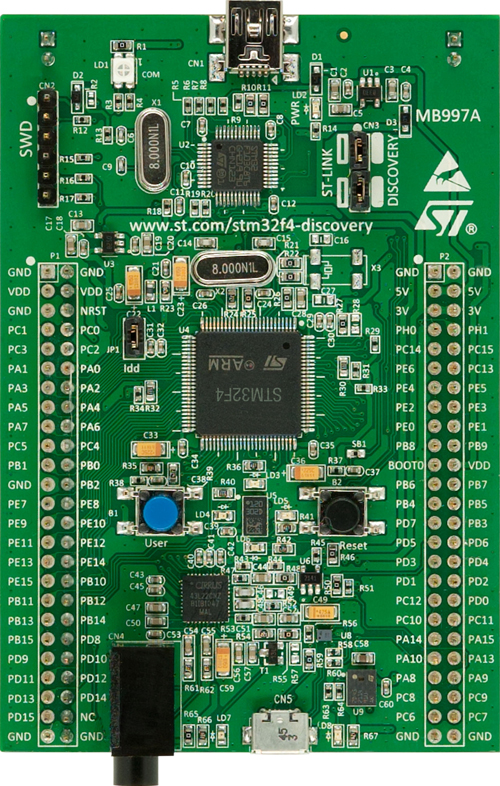
\includegraphics[scale=0.1]{../images/stm32f4_discovery.jpg}
\end{center}
\end{frame}

\subsection{Présentation eLua}
\begin{frame}
\frametitle{Introduction : Présentation eLua}
partie Elizabeth

\url{http://www.eluaproject.net/overview} +
architecture : \url{http://www.eluaproject.net/doc/v0.8/en_arch_overview.html}


la utilise le schéma et dis que notre mission c'etait d'evaluer le portage, et dire
qu'on a contacté ton James (xD) et qu'on a reussis a le faire travailler pour nous xD

C'est important je pense de le mentionner :)
\begin{center}
 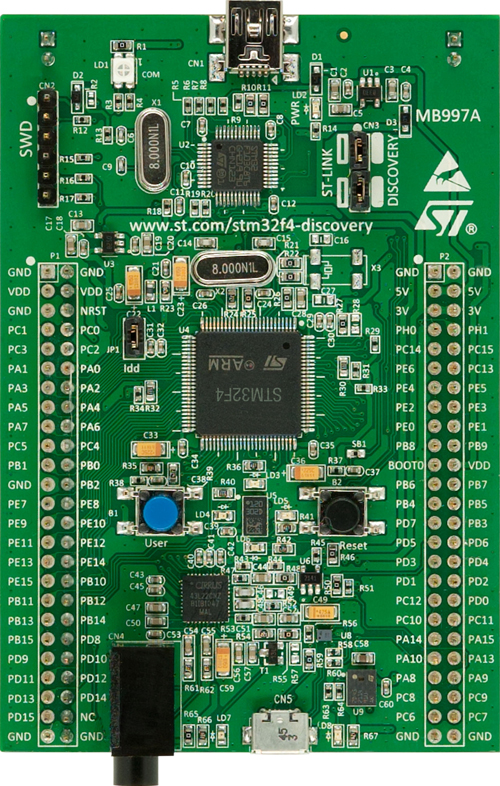
\includegraphics[scale=0.1]{../images/stm32f4_discovery.jpg}
\end{center}
\end{frame}

\section{Travail réalisé}
\subsection{Organisation du travail}
\begin{frame}
\frametitle{Organisation du travail : Agilité et Autodidacte}
\begin{enumerate}
 \item Phase I
\begin{itemize}
\item Premiers sprints assez long et peu productif
\begin{itemize}
\item Recherche d'information sur eLua et d'eventuelles portages pour STM32
\item Evaluation de la faisabilité
\item Initiation à la prgramation avec la lib stlink sur linux
\end{itemize}
\item Concertation hebdomdaire sur l'avancement
\item Discussions avec notre tuteur de stage
\end{itemize}
 \item Phase II
\begin{itemize}
\item Sprints très courts
\item Conception de l'architecure du projet
\item Developpement d'outils de travail (instalation, flash)
\item Utilisation d'un gestionnaire de version
\end{itemize}
\end{enumerate}
\end{frame}

\subsection{Arboresence du projet}
\begin{frame}
\frametitle{Arboresence du projet}
\begin{center}
 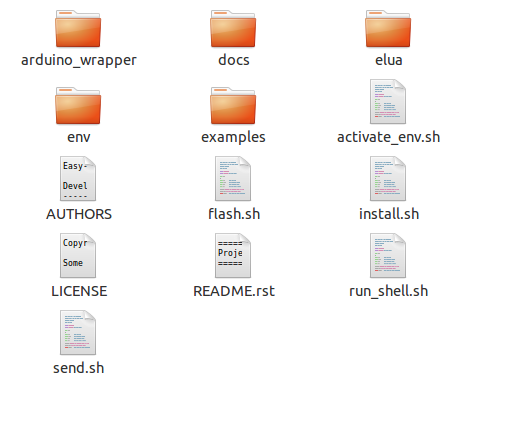
\includegraphics[scale=0.5]{../images/root_dir_project.png}
\end{center}
\end{frame}

\subsection{Fonctions portées}
\begin{frame}
\frametitle{Fonctions portées}
\begin{enumerate}
 \item Entrées/Sorties numériques
\begin{itemize}
\item pinMode() $\to$ déclarer les broches en entrée ou en sortie
\item digitalWrite() $\to$ écriture d'une valeur HIGH/LOW (1/0)
\item digitalRead() $\to$ lecture
\end{itemize}
\item Commincation Série
\begin{itemize}
\item Serial::begin() $\to$ initialiser la connexion serie
\item Serial::read()
\item Serial::write()
\item Serial::print()
\end{itemize}
\item Time
\begin{itemize}
\item millis()  $\to$ Durée d'execution du programme
\item micros()
\item delay()  $\to$ Attente passive
\item delayMicroseconds()
\end{itemize}
\end{enumerate}
\end{frame}

\subsection{Nouveaux concepts}
\begin{frame}[containsverbatim]
\frametitle{Nouveaux concepts}
\begin{enumerate}
 \item Programmation orienteé objects
 \item Lua et la métaprogrammation $\to$ Redéfinition du type ``Class``
 \item Introduction de l'objet App qui s'execute avec un contexte
\end{enumerate}

\scriptsize{\begin{lstlisting}
App = Class:new()
function App:setup()
    -- The setup function will only run once after each
    -- powerup or reset of the board
end
function App:loop()
    -- loops consecutively
end

function App:run()
    self:setup()
    while condition do
        self:loop()
    end
end
\end{lstlisting}}

\end{frame}

\begin{frame}[containsverbatim]
\frametitle{Exemple : ''Blink`` (Lua)}
\tiny{\begin{lstlisting}
require("arduino_wrapper")

function App:setup()
    self.ledpin = ORANGE_LED
    pinMode(self.ledpin, OUTPUT)
end

function App:loop()
    digitalWrite(self.ledpin, HIGH)
    delay(1000)
    digitalWrite(self.ledpin, LOW)
    delay(1000)
end

app = App:new("Blink led")
app:run()
\end{lstlisting}}
\end{frame}

\begin{frame}[containsverbatim]
\frametitle{Exemple : ''Blink`` (Arduino)}
\tiny{\begin{lstlisting}

void setup() {
  // initialize the digital pin as an output.
  // Pin 13 has an LED connected on most Arduino boards:
  pinMode(13, OUTPUT);
}

void loop() {
  digitalWrite(13, HIGH);   // set the LED on
  delay(1000);              // wait for a second
  digitalWrite(13, LOW);    // set the LED off
  delay(1000);              // wait for a second
}
\end{lstlisting}}
\end{frame}


\section{Demonstration}
\subsection{``Hello Word!''}
\begin{frame}[containsverbatim]
\frametitle{Demonstration : ``Hello Word!''}
\begin{lstlisting}
require("arduino_wrapper")
app = App:new("Hello Word!")
app:run()
\end{lstlisting}
\end{frame}

\subsection{``Blink with button''}
\begin{frame}[containsverbatim]
\frametitle{Demonstration : ``Blink with button'' avec flash}
\tiny{\begin{lstlisting}
require("arduino_wraper")

function App:setup()
    self.ledpin = RED_LED
    pinMode(self.ledpin, OUTPUT)

    self.blink = false
    self:blink_toggle()
end

function App:loop()
    if self:btn_pressed() then
        self.blink = not self.blink
        self:blink_toggle()
    end
    delay(10)
end

function App:blink_toggle()
    [...]
end
\end{lstlisting}}
\end{frame}

\subsection{``Ascii table''}
\begin{frame}[containsverbatim]
\frametitle{Demonstration : Lancement de script sans flash}
\tiny{\begin{lstlisting}
require("arduino_wrapper")

function App:setup()
    self.byte = 33
end

function App:loop()
    self:println()
    self:write(self.byte)
    self:print(", dec: " .. self.byte)
    self:print(", hex: "), self:print(self.byte, HEX)
    self:print(", oct: "), self:print(self.byte, OCT)
    self:print(", bin: "), self:print(self.byte, BIN)

    self.byte = self.byte + 1
    delay(1000)
end

app = App:new("ASCII Table ~ Character Map")
app:run()

\end{lstlisting}}
\end{frame}

\section{Conclusion}
\begin{frame}
\frametitle{Conclusion}
Couplé à la puissance d'eLua, Easy-eLua permet :
\begin{itemize}
\item Débuter dans la programmation pour l'embarqué.
\item Portabilité : Le code Lua produit est compatible avec différentes architectures supportant elua.
\item Le RAD pour l'embarqué: Prototyper et expérimenter des applications rapidement. Testez vos idées directement sans besoin de simulations ou de futures modifications.
\item Fléxibilité : Lua, langage de programmation de haut niveau, permet toute sorte d'utilisation.
\end{itemize}
\end{frame}

\begin{frame}
\frametitle{Conclusion}
\begin{center}
\huge{Des questions ?}
\end{center}
\end{frame}

\end{document}
